\documentclass[10pt,a4paper]{article}
\usepackage[utf8]{inputenc}
\usepackage{amsmath}
\usepackage{amsfonts}
\usepackage{amssymb}
\usepackage{graphicx}
\usepackage[swedish]{babel}
\usepackage[utf8]{inputenc}

\graphicspath{}

\author{
  \texttt{Sebastian Bångerius}
}

\begin{document}
\pagenumbering{gobble}

\title{Saker vi ska kunna till tentorna}
\maketitle

\cleardoublepage

\tableofcontents

\clearpage
\section{Disclaimer}
Detta dokument ser snyggt och seriöst ut för att det är skrivet i Latex. Lita inte på att allt står med. Jag är inte så seriös som jag framställer mig.

\section{Flervariabelanalys}
Vi har tagit upp områden såsom \textit{Flervariabelgränsvärden}, \textit{Partialderivator}, \textit{Partiella differetialekvationer}, \textit{Kedjeregeln} , \textit{}, \textit{Gradienter}, \textit{Funktionaldeterminanter} och \textit{Dubbel-/Trippelintegraler} samt \textit{Medelvärdessatsen}

\subsection{Triangelolikheten}
\begin{equation}
\left|x+y\right|\leq\left|x\right|+\left|y\right|
\end{equation}
\begin{flushleft}
Triangelolikheten behandlar vektorer av olika grader. Kan effektivt användas för att stänga in flervarabelfunktioner.
\end{flushleft}
\begin{center}
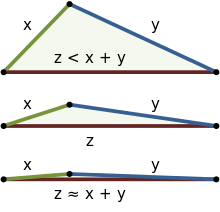
\includegraphics[scale=0.5]{triangelolikhet}
\end{center}

\subsection{Kedjeregeln}
Kedjeregeln används för att kunna bestämma derivator vid variabelbyten. I formuleringen nedan är $f$ en funktion av $x$ och $y$ enligt $f(x(u,v),y(u,v))$. Tänk på att t.ex. $x=v$ \underline{ej} medför att $\frac{\partial f}{\partial x} = \frac{\partial f}{\partial v}$.
\begin{equation}
\frac{\partial f}{\partial u}=\frac{\partial f}{\partial x}\cdot \frac{\partial x}{\partial u} + \frac{\partial f}{\partial y} \cdot \frac{\partial y}{\partial u}
\end{equation}
\begin{equation}
\frac{\partial f}{\partial v}=\frac{\partial f}{\partial x}\cdot \frac{\partial x}{\partial v} + \frac{\partial f}{\partial y} \cdot \frac{\partial y}{\partial v}
\end{equation}

\subsection{Funktionaldeterminant}
Vid variabelbyte i en integral behöver man multiplicera funktionen som skall integreras med funktionaldeterminanten. Detta kompenserar upp eventuella utsträckningar etc. som uppstått till följd av t.ex. brist på ortogonalitet i den nya basen. detta görs på följande sätt för ett variabelbyte $f(x,y) \rightarrow \tilde{f}(u,v)$.
\begin{equation}
\iint_D f(x,y)\,dx\,dy = \iint_E \tilde{f}(u,v)\cdot \frac{d(x,y)}{d(u,v)}\,du\,dv
\end{equation}
där funktionaldeterminanten $\frac{d(x,y)}{d(u,v)}$ räknas ut enligt

\begin{equation}
\frac{d(x,y)}{d(u,v)} = \left| \begin{array}{ccc}\frac{\partial x}{\partial u} & \frac{\partial x}{\partial v} \\ \frac{\partial y}{\partial u} & \frac{\partial y}{\partial v} \end{array} \right| \neq 0
\end{equation}
Minns även att 
\begin{equation}
\frac{d(x,y)}{d(u,v)} = \frac{1}{\frac{d(u,v)}{d(x,y)}}
\end{equation}


\subsection{Gradient}

\subsection{Differentierbarhet}

\subsection{Gränsvärden}

\end{document}